\documentclass{szzclass}
\usepackage{hyperref}
\usepackage{longtable}
\usepackage{booktabs}

\subject{SI2}
\code{BI-WSI-SI-24}
\topic{Projektové řízení a měření: modely SDLC, plánování krátkodobé a dlouhodobé, kategorie metrik a jejich využití, historie projektu, řízení rizik, odhady, způsob jejich tvorby a verifikace}
\providecommand{\tightlist}{%
  \setlength{\itemsep}{0pt}\setlength{\parskip}{0pt}}

\begin{document}
\tableofcontents
\newpage

\section{SDCL - Software development lifecycle}
Jedná se o množinu aktivit nutných k tomu, aby SW vznikl. SDLC definuje vztahy, prostřední, přístup, čas a jakékoli jiné vlastnosti primárních a podpůrných činností
SW inženýrství.
\subsection{Agile vs Plan-Driven}
Příklady modelů životního cyklu:
\begin{itemize}
    \item waterfall
    \item iterativní model
    \item SCRUM
\end{itemize}

Aktivity se rozdělují na Primární a Podpůrné
\begin{itemize}
    \item primární
    \begin{itemize}
        \item business modeling
        \item sběr požadavků
        \item analýza a návrh
        \item programování
        \item testování
        \item nasazení
    \end{itemize}
    \item podpurné
    \begin{itemize}
        \item projektové řízení
        \item správa prostředí
        \item změnové a konfigurační řízení
    \end{itemize}
\end{itemize}

Primární činnosti "tvoří hodnoty", probíhají do určité míry sériově (za sebou), většinou i v opakujících se cyklech.
\newline
Podpůrné činnosti probíhají stále, po celou dobu celého projektu a primární činnosti "zaobalují".

\subsection{Waterfall - dlouhodobé plánování}
Oddělené fáze:
\begin{itemize}
    \item analýza požadavků
    \item design
    \item implementace
    \item testování
    \item provoz
\end{itemize}
Výhody:
\begin{itemize}
    \item jasně definovaný plán
    \item predikovatelnost (čas, rozsah, cena)
    \item snadná koordinace práce
\end{itemize}
\newpage
Nevýhody:
\begin{itemize}
    \item nutno chápat, co se chce již na začátku
    \item reakce na změny (požadavky, termíny)
    \item rychlost dodávky (kdy nejdřív uvidí klient nějaký progress)
    \item integrace více systémů
\end{itemize}
\subsection{Iterativní - středně dlouhé plánování}
Změny oproti vodopádu:
\begin{itemize}
    \item několik verzí systému
    \item jednotlivé verze se dělají vodopádem
\end{itemize}
Výhody - stejné jako vodopád, jen má navíc :
\begin{itemize}
    \item zákazník má přístup k verzím/prototypům (vidí co dostává)
\end{itemize}
Nevýhody
\begin{itemize}
    \item nutno chápat, co se chce od začátku, možné změny do dalších verzí
\end{itemize}
\begin{figure}[h!]
    \centering
    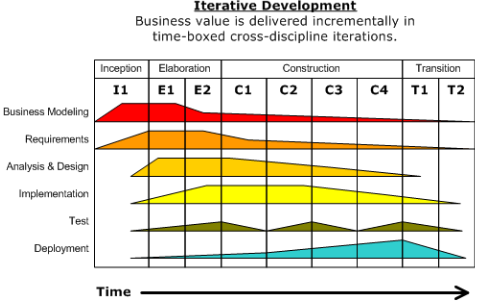
\includegraphics[width=0.7\textwidth]{topics/bi-wsi-si-24/images/iterativeDevelopment.png}
    \caption{Iterativní vývoj}
\end{figure}
\subsection{Agilní - krátkodobé plánování}
Změny oproti iterativnímu:
\begin{itemize}
    \item mnohem kratní iterace
    \item jednotlivé verze ne vždy produkční
    \item velké nároky na celý tým
    \item změna myšlení
\end{itemize}
Výhody:
\begin{itemize}
    \item rychlé
    \item nová verze brzy
    \item zpětná vazba
\end{itemize}
Nevýhody:
\begin{itemize}
    \item nutné kontinuální zapojení všech členů týmu
    \item nutný silný business vlasník
\end{itemize}
\section{Metriky}
Základní metriky:
\begin{itemize}
    \item Time (kalendářní čas - jak dlouho to bude trvat udělat)
    \item Size/Scope (jaký je rozsah)
    \begin{itemize}
        \item počet řádků kodu
        \item počet obrazovek
        \item počet tříd
        \item \dots
    \end{itemize}
    \item Effort (jak je to pracné - většinou udávané v MD)
    \item Quality (jakost - jak moc se hledí na kvalitu $\rightarrow$ výskyt chyb)
\end{itemize}
Pro zaznamenávání historie práce (projektů a jendotlivých úkolů) se používá Ticketovací systém (youtrack, github, redmine\dots).
Díky tomu se lépe odhadne časová pracnost na základě minulých dat. Podle naměřených metrik se odvíjí nabídka a cena.

\subsection{Historie}
Dokument nebo systém, který obsahuje informace a metriky z jednolivých realizovaných projektů.
Na jejich základě se lépe odhadují budoucí projekt, zpřesňovat odhady nových projektů, ekonomická hlediska a náročnost práce/údržby.
\subsection{Odhady, jejich tvorba a verifikace}
Metody odhadů:
\begin{itemize}
    \item Dekompozice zadání na elementární části
    \item odkad na základě historie
    \item odhad by měl být konzistetní a měl by být zkontrolován dalšími účastníky
    \item odhad může být proveden na základě metrik
    \item použití standartizovaných metodik, které pracují s historii
    \item lze realizovat pomocí checklistu (na které problémy se zaměřit)
\end{itemize}
\section{Řízení rizik}
Riziko je ohrožení projektu/ceny/termínu/kvality. Musí se o nich zákazník dozvědět co nejdříve, protože mohou hrát roli
při uzavření smlouvy, ceny, odhadu pracnosti\dots
U každého rizika je nutné určit:
\begin{itemize}
    \item pravděpodobnost, že nastane
    \item případný odhad
    \item jeho stav
    \item plán na snížení negativních dopadů
\end{itemize}
\end{document}